\documentclass{beamer}
\usepackage[english]{babel}
\usepackage[utf8]{inputenc}
\usepackage[T1]{fontenc}
\title{\textbf{Synthesis of Orchestrations of Transducers for Manufacturing}}
\author[Dmytro]{
\\
\vspace{5.5cm}
Dmytro Horpynchenko\\
\textit{1807584}}
\date[May 13, 2019]{}
\institute[Roma]{Università di Roma}

\usetheme[pageofpages=of, % default - any character is good: di, /
          titleline=true, % default - other choice: false
          ]{Roma}

\theoremstyle{definition}
\theoremstyle{plain}

\begin{document}
\titlepageframe % use this command to create the titlepage

\begin{frame}
Based on the paper:
\\
\textbf{Synthesis of Orchestrations of Transducers for Manufacturing}
\\
Giuseppe De Giacomo, Moshe Y. Vardi, Paolo Felli, Natasha Alechina, Brian Logan
\\
2018
\end{frame}

\begin{frame}
\frametitle{A bit of background
}
\begin{enumerate}
    \item Manufacturing as a service
    \item Adopting industry 4.0 is essential to maintain competitiveness. 
    \item Process planning   
\   item Manual $\rightarrow$ Automated
\end{enumerate}
\end{frame}

\begin{frame}
\frametitle{Previous work on the automated synthesis of process planning
}
\framesubtitle{De Silva et al. 2016 and Felli et al. 2017}
\begin{itemize}
 \item Techniques based on AI behaviour composition 
 \item In : a process recipe and a production topology 
 \item Out : a process plan controller 
 \end{itemize}
 \alert{These problems are :} 
 \begin{itemize}
     \item polynomial in the size of the topology, (exponential in the number of resources and polynomial in their size), and exponential in the size of the process recipe and number of resources
     \item Difficult to relate synthesis of controllers for manufacturing to the existing literature and tools on reactive synthesis
 \end{itemize}
 \end{frame}
 
 \begin{frame}
\frametitle{Uni-Transducer}
\begin{block}{What is a transducer? A uni-transducer?}
A transducer is a finite deterministic automaton with outputs, we consider here Mealy machines.
Uni-transducer is a machine that takes a single input and produces a single output in each state.
Model manufacturing resources and process.
\end{block}
\begin{alertblock}{Definition 1}
A (uni-)transducer $ T = ( \Sigma, \Delta, S, s_{0}, f, g) $ is a deterministic transition system with inputs and outputs, where $\Sigma$ is the input alphabet, $\Delta$ is the output alphabet, S is the set of states , $ s_{0} $ the initial state, $ f: S \times \Sigma \rightarrow S $ is the transition function (which takes a state and an input symbol and returns the successor state) and $ g: S \times \Sigma \rightarrow \Delta $ is the output function (which returns the output of the transition).
\end{alertblock}
\end{frame}
\begin{frame}{Uni-transducer example}
$ T = ( \Sigma, \Delta, S, s_{0}, f, g) $ \\
$\Sigma = \{cleansq, cleanrd, greensq, yellowrd\}$ \\
Input alphabet encodes operations \\
$\Delta = \{sqclean, rdclean, sqgreen, rdyellow, err \}$ \\
Output alphabet encodes results of operations \\
$S = {s_{0}, s_{1}, s_{2}, s_{e}}$ \\
$f(s_{0}, cleansq)=s_{1}$ 
$g(s_{0}, cleansq)=sqclean$
    
\end{frame}

\begin{frame}{Uni-transducer example}
\begin{figure}[htp]
\centering
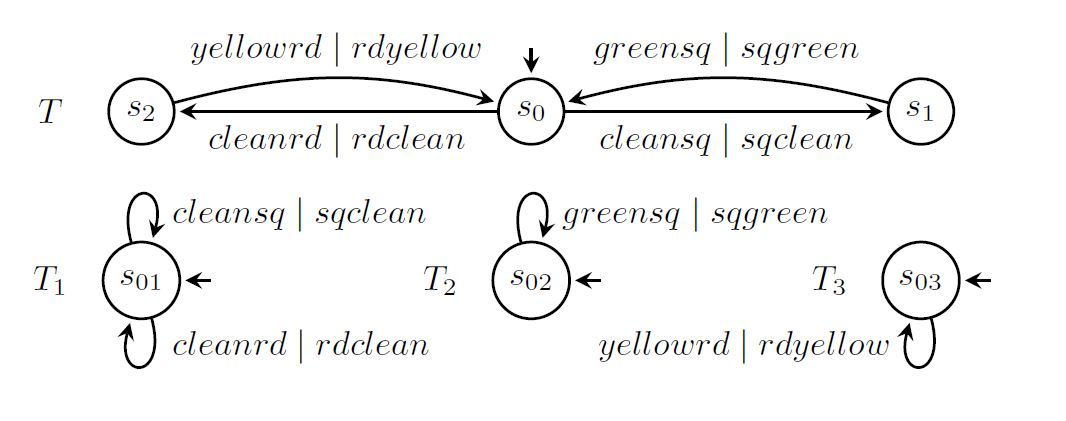
\includegraphics[width=\linewidth]{images/ex1trans.JPG}
\caption{Process recipe T and manufacturing resources $T_{1}$, $T_{2}$ and $T_{3}$}
\label{fig:ex1trans}
\end{figure}

\end{frame}
\begin{frame}{Uni-Transducer: Orchestration}
\begin{alertblock}{Definition}
Given a set of transducers $\mathnormal{T_{1},\dots,T_{m}}$ and a
production recipe transducer $\mathnormal{T}$, the orchestration problem
is the question whether there is a controller $\mathnormal{C}$ for $\mathnormal{P = T_{1} \times \dots \times T_{m}}$ which realizes $\mathnormal{T}$.
\end{alertblock}
\begin{itemize}
    \item Output sequence of $\mathrm{T}$ on input $\mathnormal{w}$: $\mathnormal{\tau^{o}_{w,T} = T^{o}(a^{0})},\dots,\mathnormal{T^{o}(a^{0}}\dots\mathnormal{a^{i})}\dots$
    \item $\mathnormal{C : \Sigma^{+}} \longrightarrow \mathrm{\{1,\dots,m\}}$
    \item The output of $\mathnormal{C}$ on $\mathnormal{P}$ over the input $\mathnormal{w}$ is $\mathnormal{\tau^{o}_{w,C} = b^{0},\dots,b^{i}},\dots$, where $\mathnormal{b^{i} = g_{h}(s^{i}_{h},a^{i})}$
    \item $\mathnormal{C}$ realizes $\mathnormal{T}$ if  $\mathnormal{\tau^{o}_{w,T} = \tau^{o}_{w,T}}$ for all $\mathnormal{w}$.
\end{itemize}
\begin{block}{Task of the controller}
Decide, at each cycle, to which resource the input should be assigned.
\end{block}    
\end{frame}
\begin{frame}{Uni-Transducer: Orchestrator Synthesis}
\begin{itemize}
    \item DFA Games
    \item $\mathrm{G} = (\mathcal{X} \times \mathcal{Y},\mathrm{Q,q_{0},\delta, F})$
    \item Win by playing forever
    \item $\mathrm{PreC}(\mathcal{E}) = \{q \in \mathrm{Q}$ | for all $\mathcal{X} \in \mathcal{Y}$ exists $\mathrm{Y} \in \mathcal{Y}$ such that $\delta(q, (\mathrm{X,Y})) \in \mathcal{E}$ \}
    \item Define $\mathrm{Win(G)}$ by greatest-fixpoint
    \item $\mathcal{T}_{G} = (\mathrm{X \times Y, Q, q_{0}, \varrho, \gamma})$
\end{itemize}
\begin{alertblock}{Theorem}
\textit{Checking whether there exists a controller $\mathnormal{C}$
for $\mathnormal{P}$ that realizes $\mathnormal{T}$ can be done by solving the safety game
$\mathnormal{G}$ defined above.}
\end{alertblock}
    
\end{frame}

\begin{frame}
\frametitle{Multi-transducers:Problem overview}
Uni-transducers are suitable only for  single pipeline processes.
Meanwhile it is essential to:
\begin{itemize}
\item Process entities in parallel
\item Split raw materials apart
\item Combine or assemble multiple items  to produce new entity type
\end{itemize}

\begin{block}{Definition}
Deterministic transition system with multiple input/output ports is called multi-port transducer or \textit{multi-transducer}
\end{block}
\end{frame}

\begin{frame}
\frametitle{Multi-transducers: Ports}
Unlike uni-transducers, all interaction between controller and transducers are done through out ports and depends on the nature of things sent within the port they are separated to:
\begin{itemize}
\item \textit{Physical} - accept/output physical objects such as parts. Physical output port can be bound only
to one (physical) input port
\item \textit{Virtual} - accept/output signals such as messages specifying that a particular operation should be performed. Virtual output port can be bound to multiple (virtual) input ports
\end{itemize}
Any type of input ports should not be bound to more than one output port.
\\
\begin{alertblock}{Note}
All input ports must have input value and all output ports must provide an output value. In case of absence there are special empty value $\epsilon$.
\end{alertblock}
\end{frame}

\begin{frame}
\frametitle{Multi-transducers: Ports}

\begin{minipage}{0.5\textwidth}
$ in_{x, y} $ - the input port $y$ of multi-transducer $T_{x}$\\
$ out_{x, y} $ - the output port $y$ of multi-transducer $T_{x}$\\
$ val(in_{x,y}), val(out_{x,y})$ - the value at the input/output port $y$ of transducer $T_{x}$\\
$ (out_{x', y'}, in_{x, y})$ - \textit{port bindings}, a connection between the output port $y'$ of multi-transducer $x'$ and input port $y$ of multi-transducer $x$\\
\end{minipage}
\hspace{0.4cm}
\begin{minipage}{0.4\textwidth}
\begin{figure}
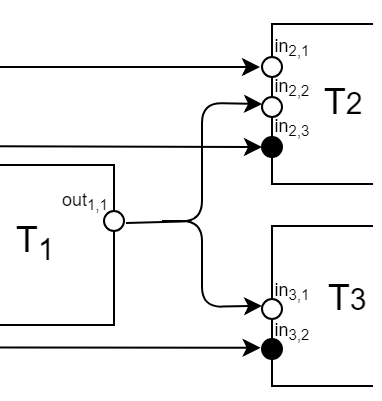
\includegraphics[scale=1]{images/mult_ports.png}
\caption{Connection example: white/black ports are virtual/physical ports respectively.}
\label{multi_ports}
\end{figure}
\end{minipage}

\end{frame}

\begin{frame}
\frametitle{Multi-transducers: Environment and routing}
Interaction with set of manufacturing resources (represented as transducers) is done using \textit{binding sets} and through an object so-called \textit{"Environment"}. Binding set is a set of port bindings that must be \textit{"legal"}: it must be consistent with requirements described above.

\begin{figure}
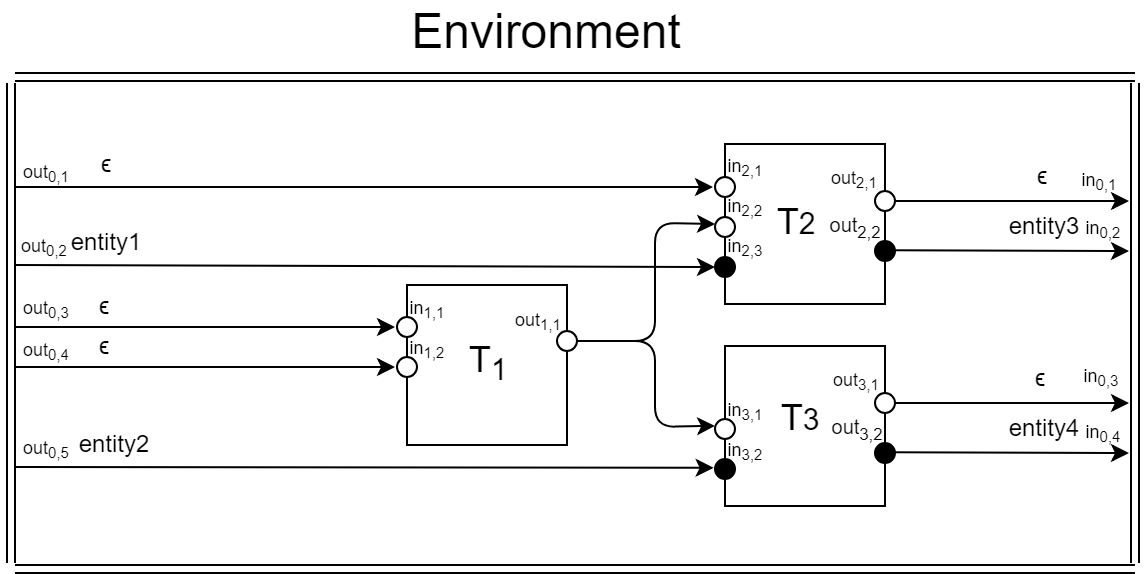
\includegraphics[scale=0.19]{images/mult_trans.png}
\caption{Example of multi-transducers binding set. Inputs and outputs that have no value use spesial $\epsilon$ value}
\end{figure}
\end{frame}

\begin{frame}
\frametitle{Multi-transducers}
Considering defined above, multi-transducer is defined as follows:
$$ T = (\Sigma, S, s_{0}, f, g, k, l) $$
,where\\
$\Sigma$ is the alphabet (of both inputs and outputs)\\
$S$ is the set of states\\
$s_{0}$ is the initial state\\
$f : S \times \Sigma^{k} \to S$ is the transition function\\
$ g : S \times \Sigma^{k} \to \Sigma^{l}$ is the output function\\
$k$ is the number of $T$'s input ports\\
$l$ is the number of $T$'s output ports
\end{frame}

\begin{frame}
\frametitle{Orchestration}
The manufacturing resources are represented as a set of multi-transducers $T_{1}, . . . , T_{m}$\\
$$T_{j} = (\Sigma, S_{j}, s_{0j}, f_{j}, g_{j}, k_{j}, l_{j})$$
The behavior of T on input $w = a^{0}a^{1}. . . $, where $a_{i} \in \Sigma_{k}$, is described by the following sequence of states and outputs:\\
$T^{s}(a^{0}) = f(s_{0}, a^{0})$\\
$T^{o}(a^{0}) = g(s_{0}, a^{0})$\\
. . .\\
$T^{s}(a^{0} . . . a^{i}) = f(T^{s}(a^{0} . . . a^{i-1}), a^{i})$\\
$T^{o}(a^{0} . . . a^{i}) = g(T^{s}(a^{0} . . . a^{i-1}), a^{i})$\\
The observable output sequence of $T$ on input $w$ is
$$\tau^{o}(w, T) = T^{o}(a^{0}) . . . T^{o}(a^{0} . . . a^{i}) . . .$$
\end{frame}

\begin{frame}
\frametitle{Orchestration}
Considering a production $P$:
$$P = T_{1} \times . . . \times T_{m}$$
a controller $C$ for $P$ is defined as:
$$C : (\Sigma_{k})^{+} \to Cntl$$
,where $Cntl$ is denoting the set of all possible port binding sets.
\\
Identically to uni-transducers case,
\begin{theorem}
$C$ realizes $T$ if $\tau^{o}(w, T) = \tau^{o}(w, C)$ for all $w$
\end{theorem}
\end{frame}

\begin{frame}
\frametitle{Orchestrator Synthesis}
Synthesizing a controller for multi-transducer setting has the same principle as in uni-transducers case:  by adopting automata-theoretic techniques and resort to solving a safety game.\\
Given the target transducer $T$ and the available transducers $\{T_{1}, . . . ,T_{m}\}$, we build the safety
game:
$$G_{multi} = (\Sigma^{k}, Cntl, Q, q_{0}, \delta)$$
where\\
$\Sigma^{k}$ is the input alphabet of the target $T$;\\
$Q = S \times S1\times . . . \times S_{m} \cup \{q_{err}\}$ is the cartesian product of the states;\\
$q0 = (s_{0,} s_{01}, . . . , s_{0m})$\\
$\delta$ is the states transition function (see next slide for definition)
\end{frame}

\begin{frame}
\frametitle{Example: Implementation of orchestration of uni-transducer setting}
As the practical part of paper analysis orchestration of uni-transducers setting was implemented in Python.
\\
\vspace{0.4cm}
Description of the target transducer and manufacturing resources must be provided as text files using special notation:
\\
\textit{state input newstate->output}
\\
\begin{block}{Read more}
Full description,python environment setup instruction, this slides and domains examples can be found on GitHub repository \url{https://github.com/dhorpynchenko/Orchestration-of-Transducers-for-Manufacturing}
\end{block}
\end{frame}

\end{document}
